\documentclass[conference]{IEEEtran}
\IEEEoverridecommandlockouts
\usepackage{cite}
\usepackage{amsmath,amssymb,amsfonts}
\usepackage{algorithmic}
\usepackage{graphicx}
\usepackage{textcomp}
\usepackage{xcolor}
\usepackage{booktabs}
\usepackage{tabularx}
\usepackage{multirow}

\begin{document}

\title{Benchmarking Next-Generation Hybrid Vision Transformers on In-The-Wild Plant Disease Detection}

\author{\IEEEauthorblockN{1\textsuperscript{st} Suman Phuyal}
\IEEEauthorblockA{\textit{Independent Researcher} \\
sfuyal59@gmail.com}
}

\maketitle

\begin{abstract}
The deployment of deep learning models for agricultural disease detection on edge devices demands architectures that are both highly accurate and computationally efficient. While traditional Convolutional Neural Networks (CNNs) like ResNet have been standard, recent advances have introduced hybrid Vision Transformers (ViTs) that blend the local feature extraction of CNNs with the global receptive fields of Transformers. This paper systematically benchmarks state-of-the-art edge-optimized hybrid models---specifically EdgeNeXt-S and FastViT-T8---against traditional CNN baselines (ResNet50 and MobileNetV4-CS) on the challenging, in-the-wild PlantDoc dataset. All models are pretrained on ImageNet-1K and fine-tuned under identical training conditions. Our results indicate that FastViT-T8 achieves the highest top-1 accuracy of 68.65\%, suggesting a favorable accuracy--efficiency trade-off over ResNet50 (+2.4\%) while requiring $7\times$ fewer parameters and $8\times$ fewer FLOPs. However, given the narrow margins between the top models, we recommend that future work validate these findings with multi-seed evaluations and additional datasets.
\end{abstract}

\begin{IEEEkeywords}
Vision Transformers, Edge Computing, Plant Disease Detection, Hybrid Architectures, FastViT, EdgeNeXt
\end{IEEEkeywords}

\section{Introduction}
Crop diseases cause significant global agricultural yield losses annually. Early detection using automated computer vision systems deployed on smartphones or edge devices (e.g., drones, Raspberry Pi) can mitigate these losses. Historically, Convolutional Neural Networks (CNNs) such as ResNet \cite{resnet} and MobileNet \cite{mobilenetv1} have dominated this space. However, they struggle to capture global contextual information efficiently.

Recently, Vision Transformers (ViTs) \cite{vit} have set new state-of-the-art records across vision tasks by utilizing self-attention mechanisms to capture long-range dependencies. Unfortunately, standard ViTs are computationally expensive and poorly suited for edge devices. To bridge this gap, hybrid architectures like EdgeNeXt \cite{edgenext} and FastViT \cite{fastvit} have emerged, combining the efficiency of CNNs with the global context of ViTs.

This study evaluates the efficacy of these next-generation hybrid models on the PlantDoc dataset \cite{plantdoc}, a highly challenging dataset composed of images taken in natural, uncontrolled environments. We benchmark four models under identical training configurations and evaluate them on accuracy, macro F1-score, parameter count, FLOPs, and CPU inference latency.

\section{Related Work}

\subsection{CNNs for Plant Disease Detection}
Extensive research has applied standard CNNs to plant disease classification, predominantly using laboratory-controlled datasets like PlantVillage \cite{plantvillage}. Models such as ResNet \cite{resnet}, EfficientNet \cite{efficientnet}, and MobileNet variants \cite{mobilenetv1} have achieved near-perfect accuracy on these curated datasets. However, when deployed in real-world scenarios with complex backgrounds, variable lighting, and occlusion, these models often suffer severe performance degradation. The introduction of the PlantDoc dataset \cite{plantdoc} provided a realistic benchmark for in-the-wild detection, revealing that models trained on controlled datasets typically lose 20--30\% accuracy on unconstrained images.

\subsection{Vision Transformers in Agriculture}
The success of Vision Transformers \cite{vit} in general computer vision has prompted their adoption for plant pathology. Thakur et al.\ \cite{thakur2022vitplant} surveyed trends in ViT-based plant disease detection, finding that Transformer-based approaches can outperform CNNs when sufficient training data is available. Borhani et al.\ \cite{borhani2022deepplant} demonstrated competitive results using standard ViTs for plant disease classification. More recently, the Swin Transformer \cite{swin} has been applied to fine-grained plant pathology tasks \cite{plantpath2021}, leveraging its hierarchical structure and shifted-window attention for multi-scale feature extraction. However, these standard Transformers remain too computationally expensive for edge deployment.

\subsection{Edge-Optimized Hybrid Architectures}
To address the computational constraints of edge deployment, architectures such as ConvNeXt \cite{convnext}, EdgeNeXt \cite{edgenext}, and FastViT \cite{fastvit} have been proposed, combining CNN efficiency with Transformer-like global context. MobileNetV4 \cite{mobilenetv4} represents the latest evolution of pure-CNN edge models. While these architectures have been extensively benchmarked on ImageNet, their comparative evaluation on specialized agricultural datasets remains limited. Our work addresses this gap by systematically benchmarking EdgeNeXt and FastViT---two of the most recent hybrid ViTs---against established CNN baselines on in-the-wild plant disease detection. We specifically select these models because: (1) they target the same latency regime ($<$25ms CPU inference), (2) they represent distinct design philosophies (SDTA vs.\ RepMixer), and (3) they have not been previously compared on agricultural data.

\section{Methodology}
\subsection{Dataset}
We utilize the PlantDoc dataset \cite{plantdoc}, which consists of 2,598 images across 28 classes of plant diseases and healthy leaves. The images are sourced from the web and captured under uncontrolled, real-world conditions with varying backgrounds, lighting, and image quality---making it significantly more challenging than laboratory-controlled alternatives like PlantVillage \cite{plantvillage}.

We split the dataset into training, validation, and test sets using an 80/10/10 stratified random split, yielding approximately 2,078 training, 260 validation, and 260 test images. The split is stratified by class to preserve the natural class distribution across all subsets.

\textbf{Data leakage considerations.} Because the PlantDoc images are web-sourced, there is a risk of near-duplicate images (e.g., the same leaf photographed from different angles) appearing across splits. While we perform image-level splitting, which is standard practice, we acknowledge that a plant-level or source-level split would provide stronger guarantees against leakage. This is a known limitation of random splitting on web-crawled datasets.

\subsection{Architectures}
We benchmark four models, spanning traditional CNNs and modern hybrids:
\begin{itemize}
    \item \textbf{ResNet50} \cite{resnet}: A deep residual CNN with 23.6M parameters, serving as the heavy baseline representing traditional architectures.
    \item \textbf{MobileNetV4-CS} \cite{mobilenetv4}: The latest generation pure-CNN edge model employing Universal Inverted Bottleneck blocks, offering the smallest footprint (2.5M parameters) and lowest latency.
    \item \textbf{EdgeNeXt-S} \cite{edgenext}: A hybrid CNN-Transformer architecture that introduces Split Depth-wise Transpose Attention (SDTA) to efficiently capture cross-channel and spatial context with minimal overhead.
    \item \textbf{FastViT-T8} \cite{fastvit}: An ultra-fast hybrid architecture leveraging structural reparameterization via RepMixer. During training, the model uses multi-branch convolutional token mixing blocks that are mathematically fused into single, efficient convolution layers at inference time. This reparameterization reduces latency without sacrificing the representational capacity gained during training.
\end{itemize}

\subsection{Experimental Setup}
All models are initialized with ImageNet-1K pretrained weights from the \texttt{timm} library and fine-tuned on PlantDoc. This constitutes transfer learning, not training from scratch. Table~\ref{tab:hyperparams} summarizes the complete training configuration.

\begin{table}[htbp]
\caption{Training Hyperparameters}
\label{tab:hyperparams}
\begin{center}
\begin{tabular}{ll}
\toprule
\textbf{Hyperparameter} & \textbf{Value} \\
\midrule
Optimizer & AdamW \\
Learning rate & $1 \times 10^{-4}$ \\
Weight decay & $1 \times 10^{-4}$ \\
LR schedule & Cosine Annealing \\
Epochs & 50 \\
Batch size & 32 \\
Input resolution & $224 \times 224$ \\
Label smoothing & 0.1 \\
Mixup $\alpha$ & 0.2 \\
Mixed precision & AMP (FP16) \\
Model selection & Best validation loss \\
Pretrained weights & ImageNet-1K (\texttt{timm}) \\
\midrule
\multicolumn{2}{l}{\textit{Data Augmentations (training only)}} \\
\midrule
\multicolumn{2}{l}{RandomResizedCrop(224)} \\
\multicolumn{2}{l}{RandomHorizontalFlip} \\
\multicolumn{2}{l}{RandomVerticalFlip} \\
\multicolumn{2}{l}{ColorJitter(0.2, 0.2, 0.2, 0.1)} \\
\multicolumn{2}{l}{ImageNet normalization} \\
\bottomrule
\end{tabular}
\end{center}
\end{table}

All models are trained under identical conditions to ensure a fair comparison. Evaluation uses center-cropped $224 \times 224$ images with ImageNet normalization only (no augmentations). CPU inference latency is measured as the average over 50 forward passes after a 10-iteration warmup, using a single-image batch on CPU.

\section{Results and Discussion}

\begin{table}[htbp]
\caption{Benchmark Results on PlantDoc Dataset}
\label{tab:results}
\begin{center}
\begin{tabularx}{\columnwidth}{l *{5}{X}}
\toprule
\textbf{Model} & \textbf{Acc. (\%)} & \textbf{F1} & \textbf{Params (M)} & \textbf{FLOPs (G)} & \textbf{Lat. (ms)} \\
\midrule
FastViT-T8 & \textbf{68.65} & \textbf{0.66} & 3.28 & 0.54 & 20.92 \\
EdgeNeXt-S & 68.25 & 0.65 & 5.29 & 0.97 & 21.32 \\
ResNet50 & 66.27 & 0.64 & 23.57 & 4.11 & 47.89 \\
MobileNetV4-CS & 60.71 & 0.61 & \textbf{2.53} & \textbf{0.19} & \textbf{8.74} \\
\bottomrule
\end{tabularx}
\end{center}
\end{table}

\subsection{Performance Analysis}
As shown in Table~\ref{tab:results}, FastViT-T8 achieves the highest top-1 accuracy (68.65\%) and macro F1-score (0.66) among the four models evaluated. It outperforms the ResNet50 baseline by 2.4 percentage points while using only 14\% of its parameters (3.28M vs.\ 23.57M) and 13\% of its FLOPs (0.54G vs.\ 4.11G). Furthermore, when analyzing inference speed (see Fig.~\ref{fig:acc_lat}), FastViT executes more than twice as fast as ResNet50 on CPU.

EdgeNeXt-S also demonstrates competitive performance, surpassing ResNet50 in accuracy by 2.0 percentage points while maintaining a parameter count more than $4\times$ smaller. Notably, the margin between FastViT-T8 and EdgeNeXt-S is only 0.40 percentage points, suggesting that both hybrid architectures perform similarly on this task. A multi-seed evaluation would be needed to determine whether this difference is statistically significant.

MobileNetV4-CS achieves the lowest latency (8.74ms) and smallest model size (2.53M parameters) but at a substantial accuracy cost, trailing FastViT-T8 by nearly 8 percentage points. This suggests that for the complex, in-the-wild images in PlantDoc, the global context provided by hybrid attention mechanisms offers a meaningful advantage over pure convolutions.

\subsection{Per-Class Analysis and Class Imbalance}
While FastViT-T8 and EdgeNeXt-S achieve the highest overall accuracy, their macro F1-scores (0.66 and 0.65, respectively) are lower than their accuracy, indicating uneven per-class performance. The PlantDoc dataset is naturally imbalanced, and these results suggest that the models may perform better on well-represented classes while struggling with rare minority classes.

Interestingly, MobileNetV4-CS shows a smaller gap between its accuracy (60.71\%) and macro F1-score (0.61), suggesting that pure CNNs may exhibit more uniform per-class performance, albeit at a lower overall accuracy ceiling. A per-class F1-score breakdown and confusion matrix analysis (provided in our supplementary results) offer further insight into which specific disease classes are most challenging.

\subsection{Limitations and Future Work}
This study has several limitations that should be addressed in future work:

\textbf{Single dataset.} All results are evaluated on PlantDoc only. While PlantDoc provides a realistic in-the-wild benchmark, generalization to other agricultural datasets (e.g., PlantVillage \cite{plantvillage}, Plant Pathology 2021 \cite{plantpath2021}) remains to be validated.

\textbf{Single training run.} The current results are from a single training run with a fixed random seed. Given the narrow margins between models (0.40 percentage points between FastViT-T8 and EdgeNeXt-S), multi-seed evaluations with reported mean $\pm$ standard deviation would provide stronger statistical evidence for model ranking.

\textbf{Training recipe ablation.} We apply Mixup ($\alpha$=0.2) and label smoothing (0.1) uniformly to all models. An ablation study isolating the contribution of these regularization techniques from the architectural differences would strengthen the analysis.

\textbf{Class imbalance mitigation.} While a 68.65\% accuracy is promising for edge deployment on complex in-the-wild data, it is not yet sufficient for reliable commercial deployment. Future work should explore Focal Loss or class-weighted Cross-Entropy to improve performance on rare minority classes, thereby driving the macro F1-score closer to the top-1 accuracy.

\begin{figure}[htbp]
\centerline{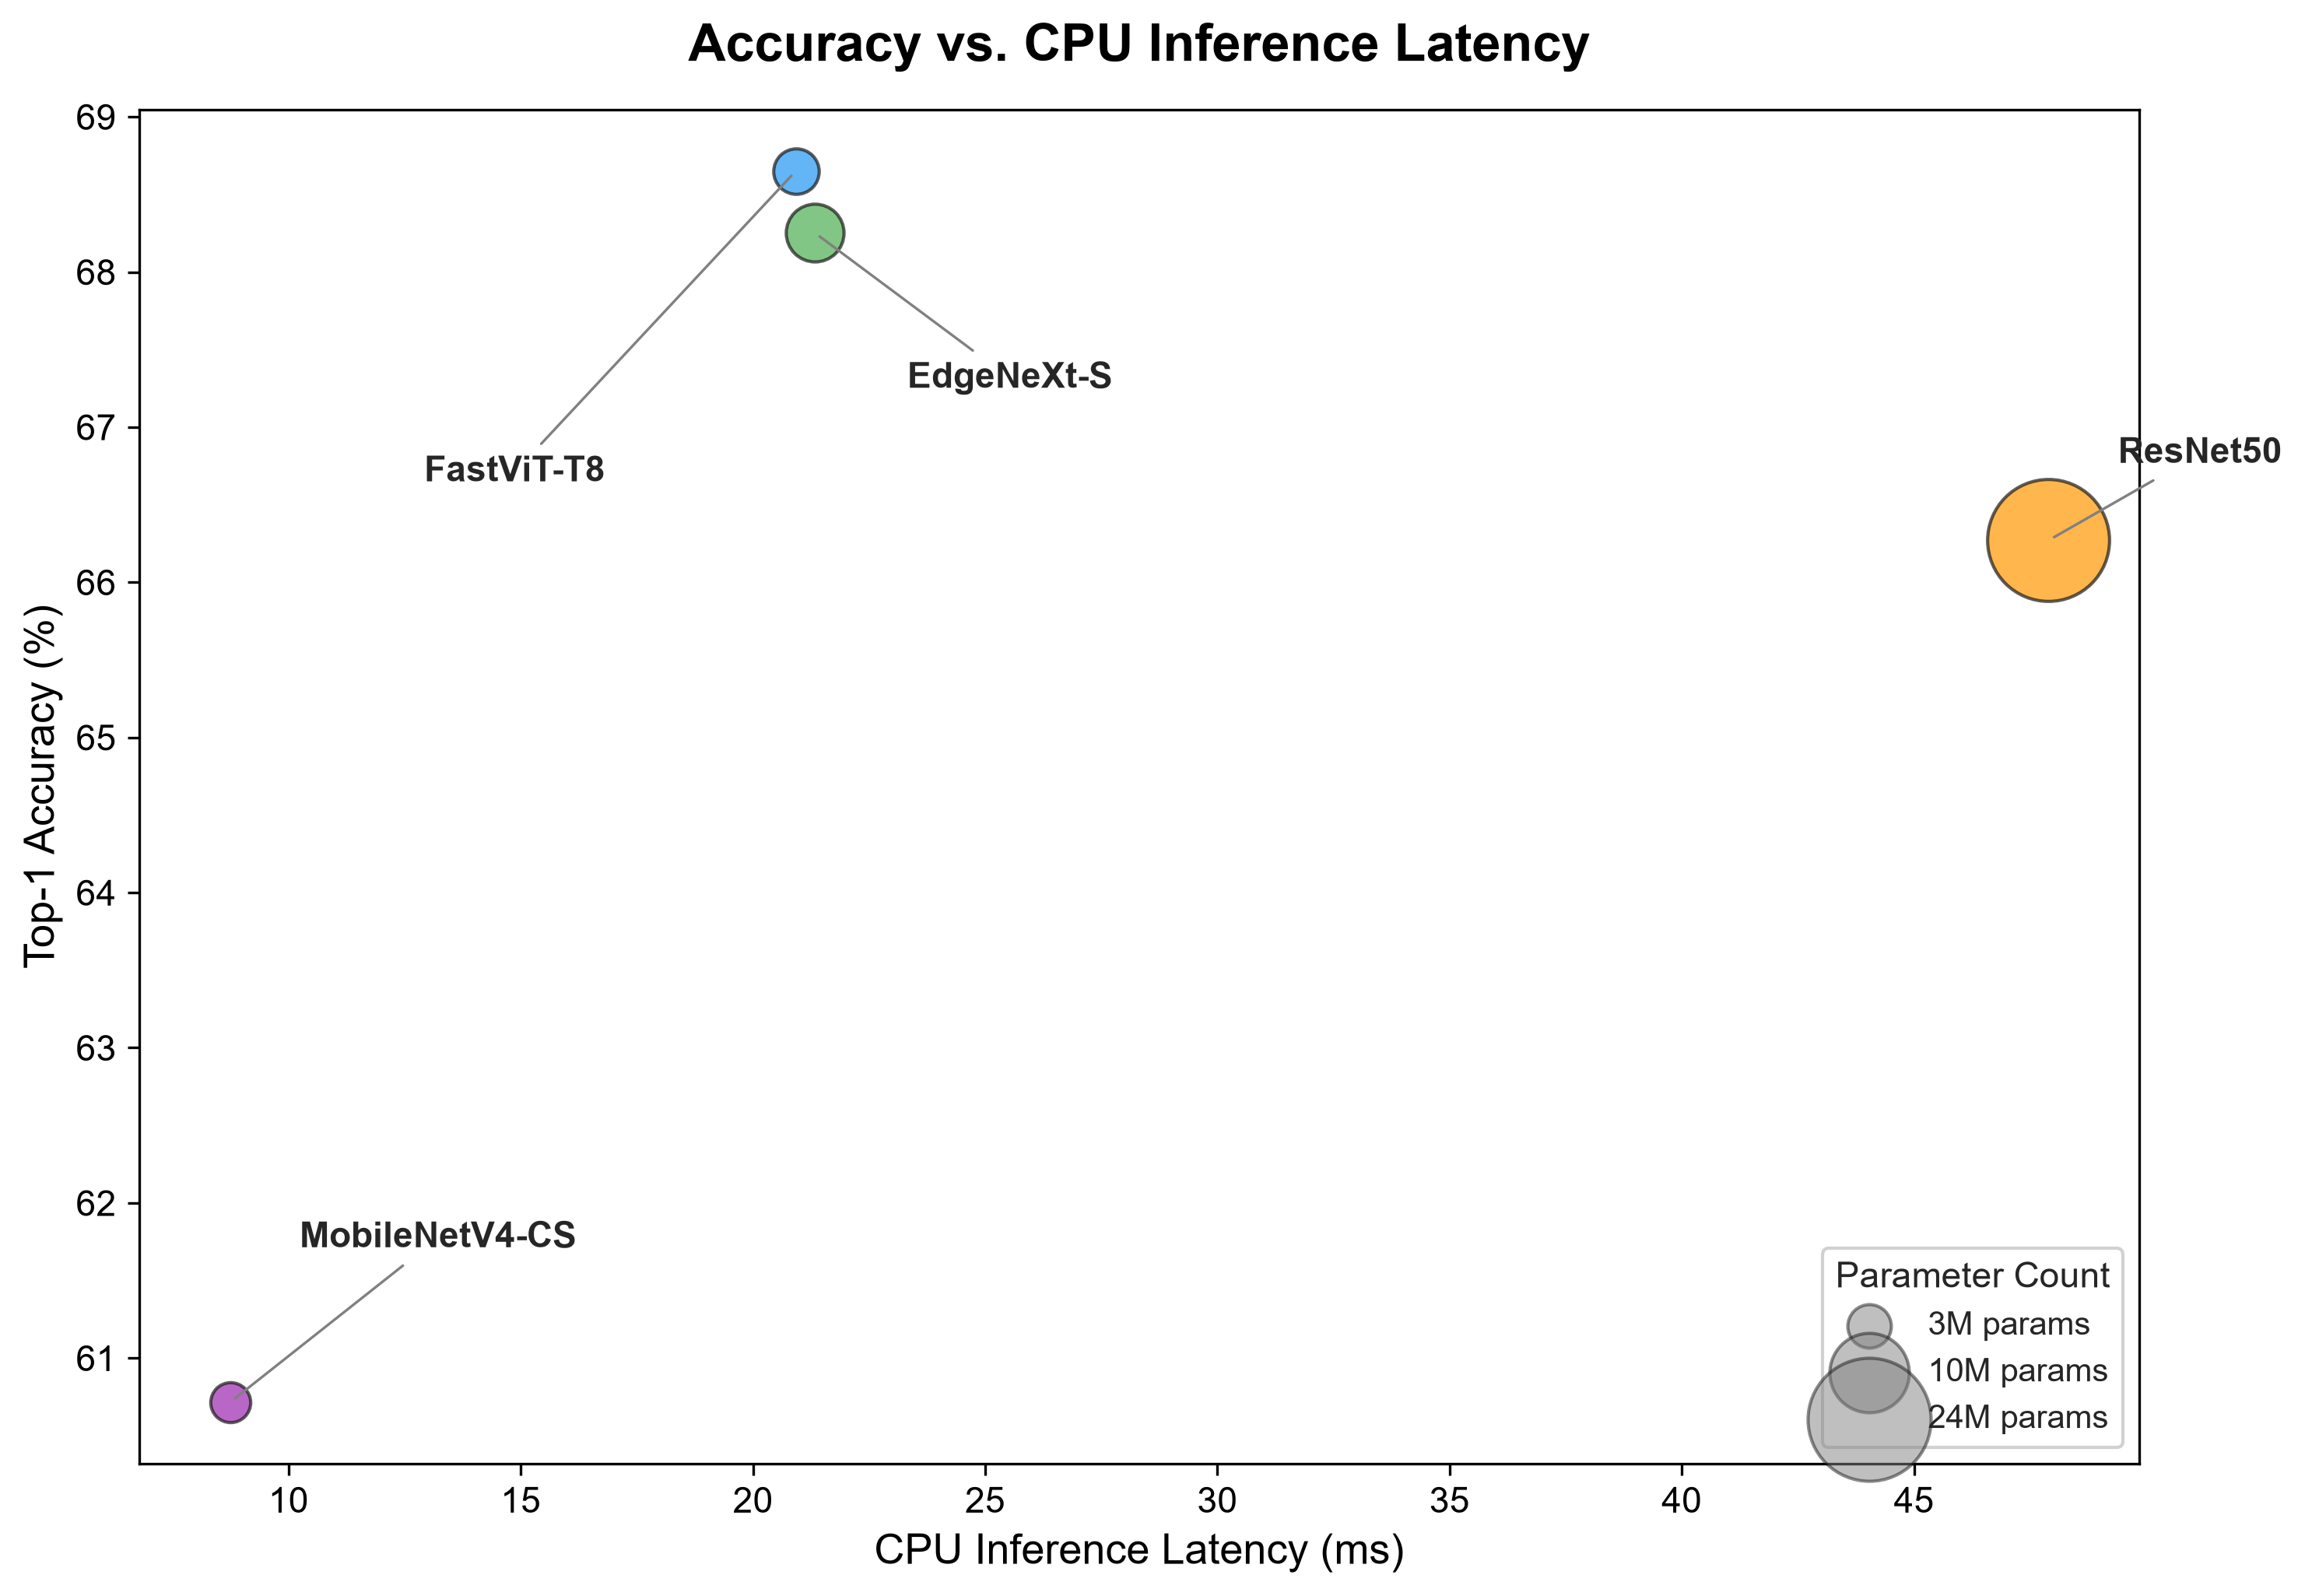
\includegraphics[width=\columnwidth]{figures/accuracy_vs_latency.png}}
\caption{Accuracy vs.\ CPU Latency. Bubble size represents parameter count.}
\label{fig:acc_lat}
\end{figure}

\begin{figure}[htbp]
\centerline{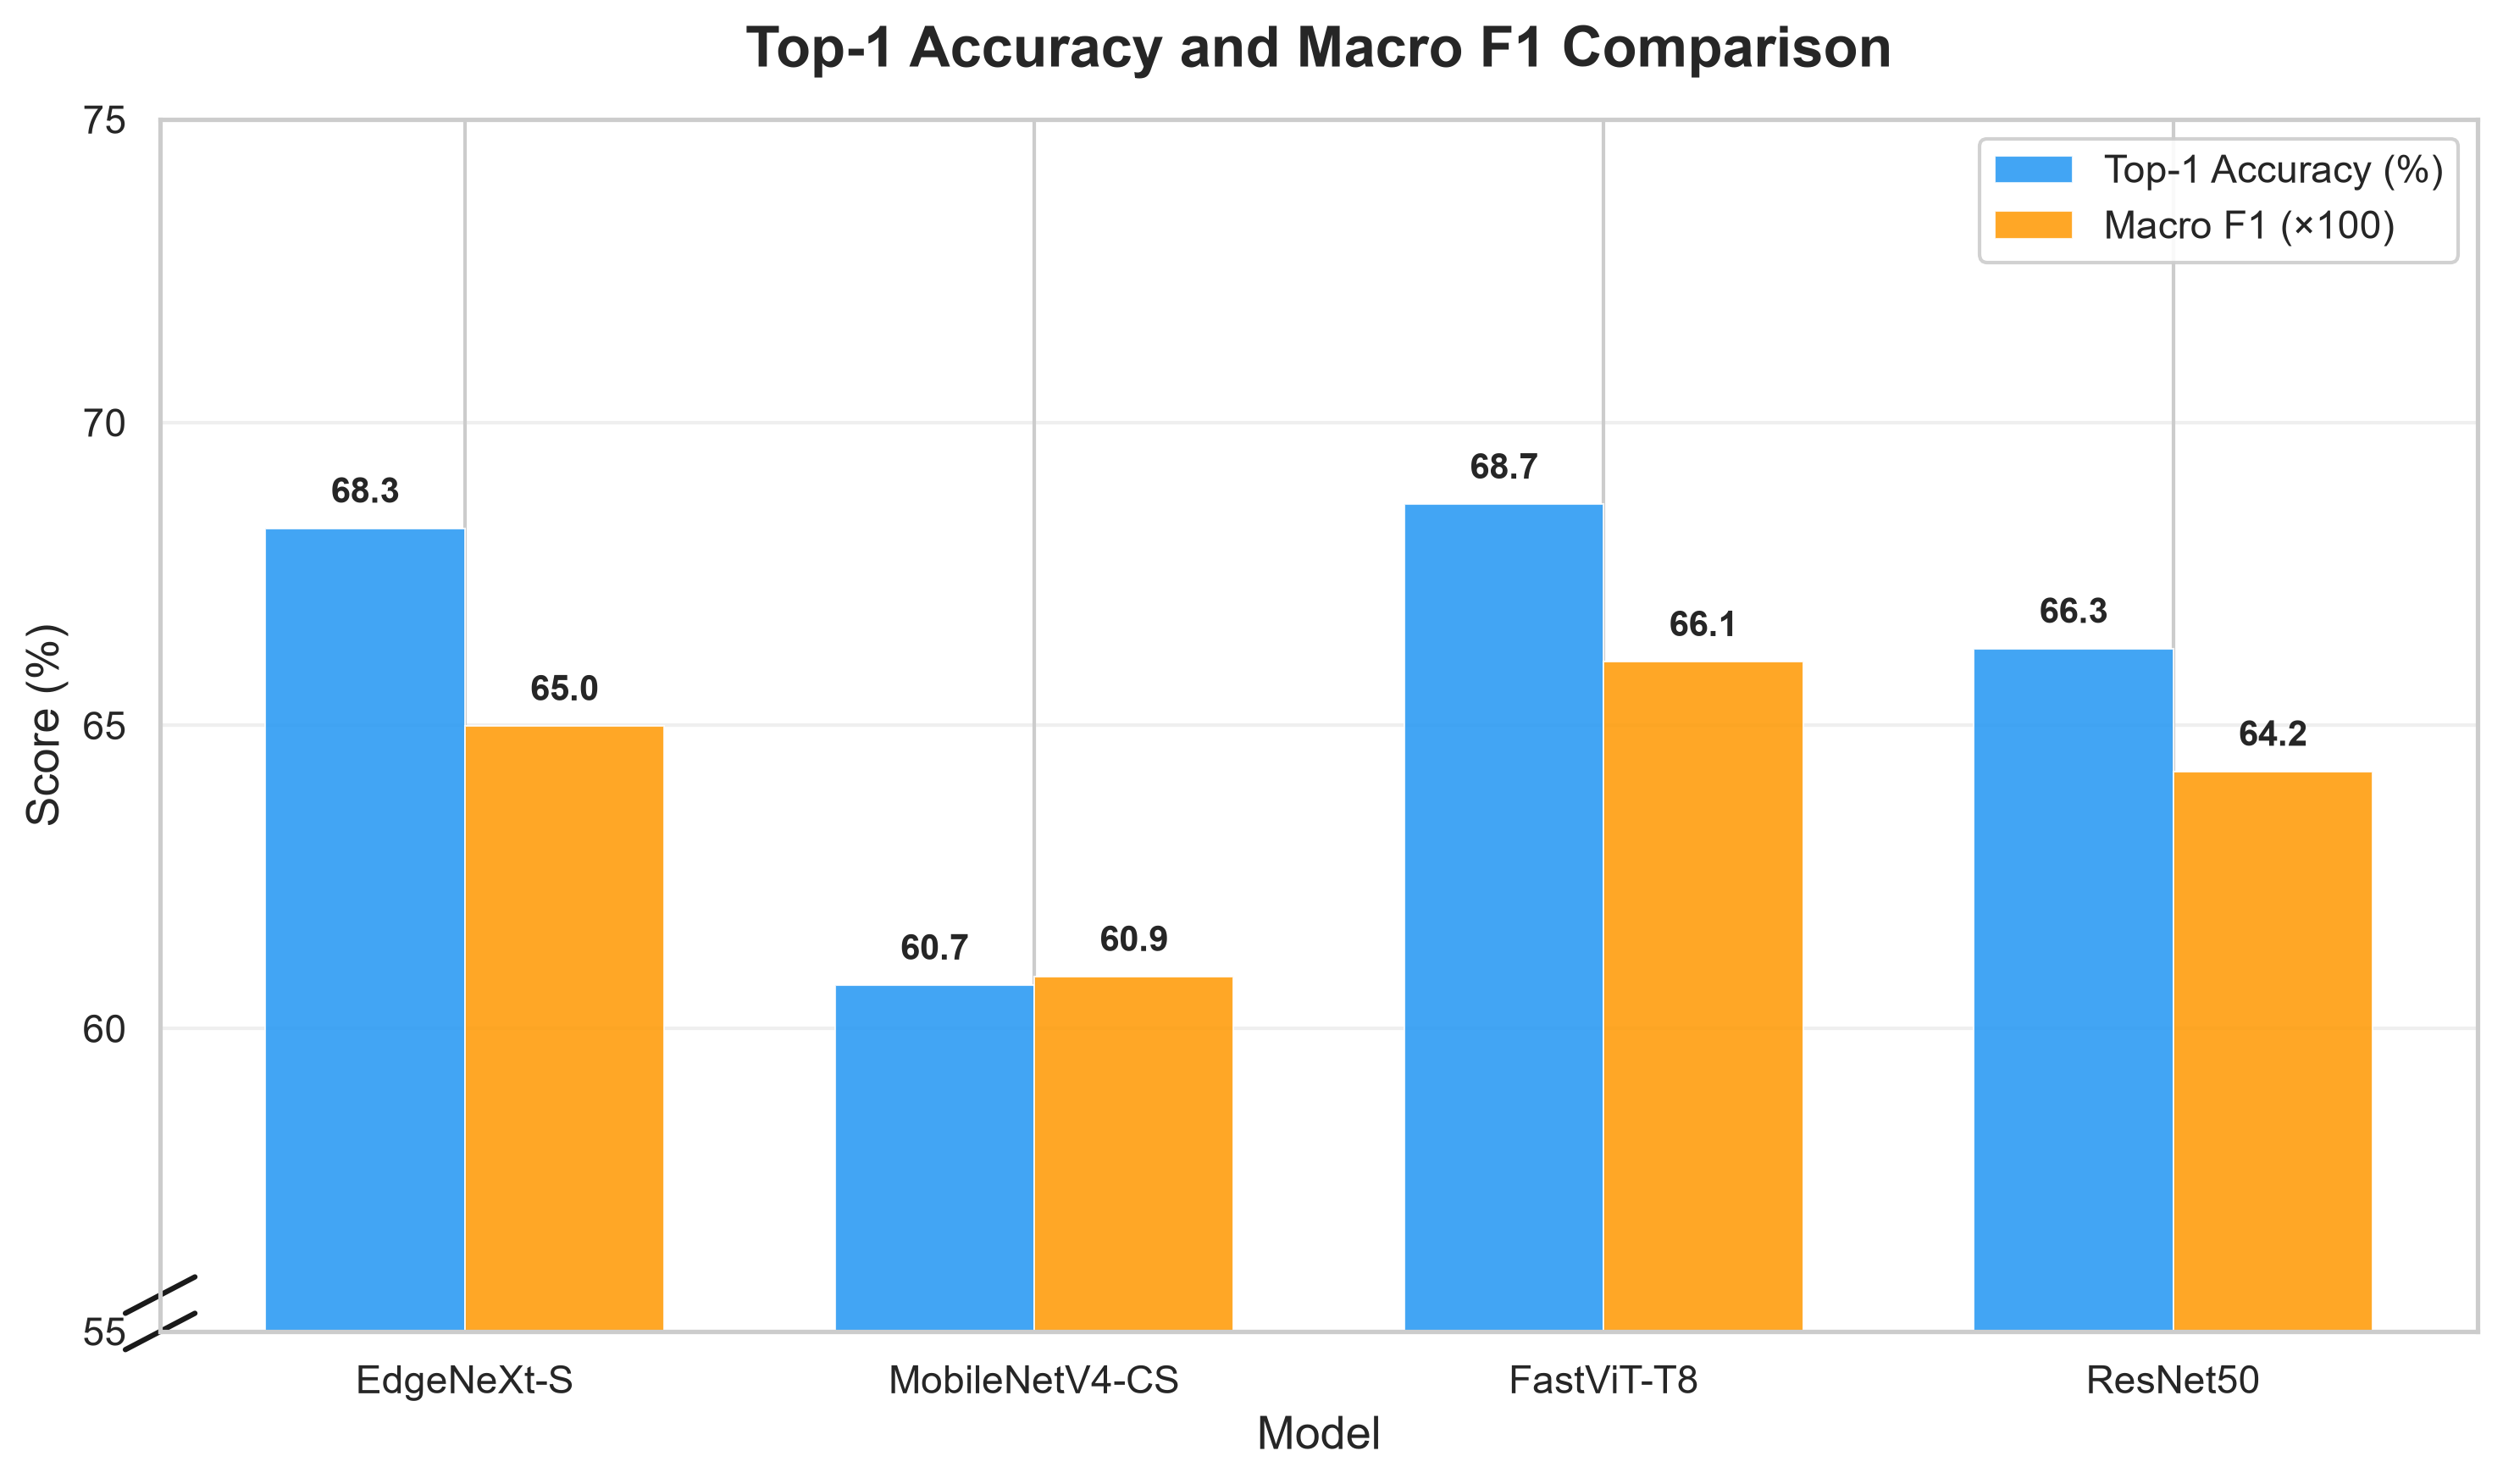
\includegraphics[width=\columnwidth]{figures/metrics_comparison.png}}
\caption{Comparison of Top-1 Accuracy and Macro F1 across models. Y-axis begins at 55\% to emphasize inter-model differences.}
\label{fig:metrics}
\end{figure}

\section{Conclusion}
This study benchmarks next-generation hybrid Vision Transformers against traditional CNN baselines for edge-based agricultural disease detection on the in-the-wild PlantDoc dataset. Our results suggest that hybrid architectures, particularly FastViT-T8 and EdgeNeXt-S, offer a favorable trade-off between accuracy and computational efficiency compared to ResNet50 and MobileNetV4-CS. FastViT-T8 achieves the best overall accuracy (68.65\%) and macro F1-score (0.66) while maintaining a compact model size suitable for edge deployment.

However, given the narrow performance margins between the hybrid models and the evaluation on a single dataset with a single training run, we caution against overgeneralization. Future work should incorporate multi-seed evaluations, additional datasets, and class imbalance mitigation strategies to provide stronger evidence for deployment recommendations.

\bibliographystyle{IEEEtran}
\bibliography{references}

\end{document}
